\section{Staff Assistant}
\subsection*{(a)}
The event $E_i$ is defined as the event that the $i^{th}$ candidate is the best and that we hire him.
We define a few more events as follows.
\begin{align*}
	B_i & : \text{The $i^{th}$ candidate is the best} \\
	H_i & : \text{We hire the $i^{th}$ candidate}     \\
	E_i & : B_i \cap H_i                              \\
	E   & : \text{We hire the best candidate}
\end{align*}
Using the definition of conditional probability, we can write the probability of event $E_i$ as follows.
\begin{align}\label{eq:staff1}
	\Pr(E_i) & = \Pr(B_i \cap H_i)         \nonumber \\
	         & = \Pr(H_i \mid B_i)\Pr(B_i)
\end{align}
Since exactly one candidate can be the best, we can calculate the probability of event $B_i$ as follows.
\begin{align}\label{eq:staff2}
	\Pr(B_i) & = \frac{1}{n}
\end{align}
If $i\leq m$ then we know that $i^{th}$ candidate cannot be hired. Otherwise, given $B_i$, we know that $i^{th}$ candidate is the best, so he/she is automatically better than the first $m$ candidates interviewed.
The only extra condition, to have them hired is that the candidates $m+1$ to $i-1$ (both inclusive) are not better than the first $m$ candidates.
Or in other words, the best among the first $i-1$ candidates is in the first $m$ candidates.
\begin{align}\label{eq:staff3}
	\Pr(H_i \mid B_i) & =
	\begin{cases}
		0             & i\leq m \\
		\frac{m}{i-1} & i > m
	\end{cases}
\end{align}
From equations (\ref{eq:staff1}), (\ref{eq:staff2}), and (\ref{eq:staff3}), we get.
\begin{align}\label{eq:staff4}
	\Pr(E_i) & =
	\begin{cases}
		0                             & i\leq m \\
		\frac{m}{i-1}\cdot\frac{1}{n} & i > m
	\end{cases}
\end{align}
Some candidate $i$ must be the best, so we can calculate the probability of event $E$ as the sum of the probabilities of all the events $E_i$.
From equation (\ref{eq:staff4}), we get.
\begin{align}\label{eq:PrE}
	\Pr(E) & = \sum_{j = 1}^{n} \Pr(E_i)                    \nonumber \\
	       & = \frac{m}{n} \sum_{j = m+1}^{n} \frac{1}{j-1}
\end{align}

\subsection{(b)}
Consider the function
\[f(x) = \frac{1}{m+x-1}\]
\begin{figure}[H]
	\centering
	\begin{subfigure}{.34\textwidth}
		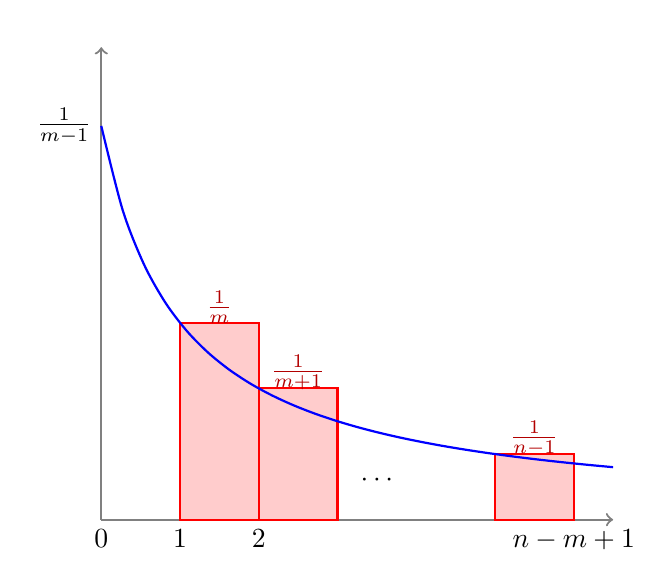
\begin{tikzpicture}
			% Axes
			\draw[->, thick, color=gray] (0,0) -- (6.5,0) node[right] {};
			\draw[->, thick, color=gray] (0,0) -- (0,6) node[above] {};

			% Rectangles
			\fill[red!20] (1,0) rectangle (2,2.5);
			\fill[red!20] (2,0) rectangle (3,1.67);
			\fill[red!20] (5,0) rectangle (6,0.8333);
			\draw[red, thick] (1,2.5) -- (2,2.5) -- (2,0) -- (1,0) -- cycle;
			\draw[red, thick] (2,1.67) -- (3,1.67) -- (3,0) -- (2,0) -- cycle;
			\draw[red, thick] (5,0.8333) -- (6,0.8333) -- (6,0) -- (5, 0) -- cycle;

			% Curve
			\draw[domain=0:6.5, smooth, variable=\x, thick, color=blue] plot ({\x}, {5/(\x + 1)});

			% Labels for rectangles
			\node[red!70!black] at (1.5,2.7) {$\frac{1}{m}$};
			\node[red!70!black] at (2.5,1.87) {$\frac{1}{m+1}$};
			\node[red!70!black] at (5.5,1.0333) {$\frac{1}{n-1}$};

			% x-axis labels
			\node[below] at (1,0) {1};
			\node[below] at (2,0) {2};
			\node[below] at (6,0) {$n-m+1$};
			\node[below] at (0,0) {0};

			% y-axis labels
			\node[left] at (0,5) {$\frac{1}{m-1}$};

			% Dots
			\node at (3.5,0.5) {$\cdots$};
		\end{tikzpicture}
		\caption{Graph of $f(x)$. The rectangles constitute the required summation, and is greater than the area under the curve from $x=1$ to $x=n-m+1$.}
		\label{fig:lower_bound}
	\end{subfigure}
	\hfill
	\begin{subfigure}{.34\textwidth}
		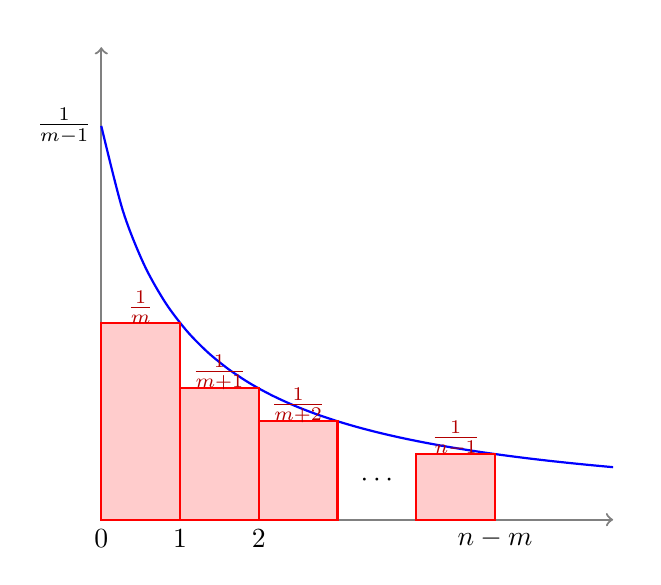
\begin{tikzpicture}
			% Axes
			\draw[->, thick, color=gray] (0,0) -- (6.5,0) node[right] {};
			\draw[->, thick, color=gray] (0,0) -- (0,6) node[above] {};

			% Curve
			\draw[domain=0:6.5, smooth, variable=\x, thick, color=blue] plot ({\x}, {5/(\x + 1)});

			% Rectangles
			\fill[red!20] (0,0) rectangle (1,2.5);
			\fill[red!20] (1,0) rectangle (2,1.67);
			\fill[red!20] (2,0) rectangle (3,1.25);
			\fill[red!20] (4,0) rectangle (5,0.8333);
			\draw[red, thick] (0,2.5) -- (1,2.5) -- (1,0) -- (0,0) -- cycle;
			\draw[red, thick] (1,1.67) -- (2,1.67) -- (2,0) -- (1,0) -- cycle;
			\draw[red, thick] (2,1.25) -- (3,1.25) -- (3,0) -- (2,0) -- cycle;
			\draw[red, thick] (4,0.8333) -- (5,0.8333) -- (5,0) -- (4, 0) -- cycle;

			% Labels for rectangles
			\node[red!70!black] at (0.5,2.7) {$\frac{1}{m}$};
			\node[red!70!black] at (1.5,1.87) {$\frac{1}{m+1}$};
			\node[red!70!black] at (2.5,1.45) {$\frac{1}{m+2}$};
			\node[red!70!black] at (4.5,1.033) {$\frac{1}{n-1}$};

			% x-axis labels
			\node[below] at (1,0) {1};
			\node[below] at (2,0) {2};
			\node[below] at (5,0) {$n-m$};
			\node[below] at (0,0) {0};

			% y-axis labels
			\node[left] at (0,5) {$\frac{1}{m-1}$};

			% Dots
			\node at (3.5,0.5) {$\cdots$};
		\end{tikzpicture}
		\caption{Graph of $f(x)$. The rectangles constitute the required summation, and is less than the area under the curve from $x=0$ to $x=n-m$.}
		\label{fig:upper_bound}
	\end{subfigure}
	\caption{\label{fig:riemann} $f(x)$ and Riemann Sums}
\end{figure}
From \Cref{fig:lower_bound}, we can see that the total area of the red rectangles is equal to the summation $\sum_{j=m+1}^n\frac{1}{j-1}$, and that area is greater than the area under the curve $f(x)$ from $x=1$ to $x=n-m+1$.
So, we can obtain a lower bound for the summation.
\begin{align}
	\sum_{j=m+1}^n\frac{1}{j-1} & \geq \int_{1}^{n-m+1} f(x) \, dx \nonumber         \\
	                            & = \int_{1}^{n-m+1} \frac{1}{m+x-1} \, dx \nonumber \\
	                            & = \ln(m+x-1)\Big|_1^{n-m+1} \nonumber              \\
	                            & = \ln(n) - \ln(m) \label{eq:lower_bound}
\end{align}
Similarly, from \Cref{fig:upper_bound}, we can see that the total area of the red rectangles is equal to the summation $\sum_{j=1}^n\frac{1}{j-1}$, and that area is less than the area under the curve $f(x)$ from $x=0$ to $x=n-m$.
So, we can obtain an upper bound for the summation.
\begin{align}
	\sum_{j=m+1}^n\frac{1}{j-1} & \leq \int_{0}^{n-m} f(x) \, dx \nonumber         \\
	                            & = \int_{0}^{n-m} \frac{1}{m+x-1} \, dx \nonumber \\
	                            & = \ln(m+x-1)\Big|_0^{n-m} \nonumber              \\
	                            & = \ln(n-1) - \ln(m-1) \label{eq:upper_bound}
\end{align}
From equations (\ref{eq:PrE}), (\ref{eq:lower_bound}) and (\ref{eq:upper_bound}), we get
\begin{align}\label{eq:final_bound}
	\frac{m}{n} \left(\ln(n) - \ln(m)\right) \leq \Pr(E) \leq \frac{m}{n} \left(\ln(n-1) - \ln(m-1)\right)
\end{align}

\subsection{(c)}
First, we define $x=\frac{m}{n}$, and since $m$ and $n$ positive integers where $n \geq m$, we have $0< x\leq 1$. Then, the function that we wish to maximise becomes
\begin{align}\label{eq:funcg}
	\frac{m}{n} \left(\ln(n) - \ln(m)\right) & = \frac{m}{n}\ln\left(\frac{n}{m}\right) \nonumber  \\
	                                         & = -\frac{m}{n}\ln\left(\frac{m}{n}\right) \nonumber \\
	                                         & = -x\ln(x) = g(x)
\end{align}
Now, our goal is to maximise $g(x)$. We can do this by taking the derivative of $g(x)$ with respect to $x$ and setting it to zero.
First, we calculate the derivative of $g(x)$.
\begin{align*}
	\diff{g(x)}{x} & = -\ln(x) - \frac{x}{x} \\
	               & = -\ln(x) - 1
\end{align*}
Next, we set the derivative to zero and solve for $x$.
\begin{align*}
	\diff{g(x)}{x} & = 0           \\
	-\ln(x) - 1    & = 0           \\
	\ln(x)         & = -1          \\
	x              & = \frac{1}{e}
\end{align*}
To verify that this is a maxima, we take the second derivative of $g(x)$.
\begin{align*}
	\diff[2]{g(x)}{x} & = \diff{\left(-\ln(x)-1\right)}{x} \\
	                  & = -\frac{1}{x}                     \\
	                  & < 0 \text{\,\,\,  (since $x>0$)}
\end{align*}
The second derivative is negative, so the function has a maxima at $x=\frac{1}{e}$.
Which means that $m = \frac{n}{e}$ is the optimal value of $m$.
Next, we compute the value of $g(x)$ at $x = \frac{1}{e}$, which is the same as the value of $\frac{m}{n}\left(\ln(n)-\ln(m)\right)$ at $m=\frac{n}{e}$.
\begin{align}\label{eq:optimal_value}
	g\left(\frac{1}{e}\right) & = -\frac{1}{e}\ln\left(\frac{1}{e}\right) \nonumber \\
	                          & = \frac{\ln(e)}{e}                        \nonumber \\
	                          & = \frac{1}{e}
\end{align}
From equations (\ref{eq:final_bound}), (\ref{eq:funcg}) and (\ref{eq:optimal_value}), we get
\[\Pr(E) \geq \frac{1}{e}\]

